% Options for packages loaded elsewhere
\PassOptionsToPackage{unicode}{hyperref}
\PassOptionsToPackage{hyphens}{url}
\PassOptionsToPackage{dvipsnames,svgnames,x11names}{xcolor}
%
\documentclass[
  letterpaper,
  DIV=11,
  numbers=noendperiod]{scrartcl}

\usepackage{amsmath,amssymb}
\usepackage{lmodern}
\usepackage{setspace}
\usepackage{iftex}
\ifPDFTeX
  \usepackage[T1]{fontenc}
  \usepackage[utf8]{inputenc}
  \usepackage{textcomp} % provide euro and other symbols
\else % if luatex or xetex
  \usepackage{unicode-math}
  \defaultfontfeatures{Scale=MatchLowercase}
  \defaultfontfeatures[\rmfamily]{Ligatures=TeX,Scale=1}
\fi
% Use upquote if available, for straight quotes in verbatim environments
\IfFileExists{upquote.sty}{\usepackage{upquote}}{}
\IfFileExists{microtype.sty}{% use microtype if available
  \usepackage[]{microtype}
  \UseMicrotypeSet[protrusion]{basicmath} % disable protrusion for tt fonts
}{}
\makeatletter
\@ifundefined{KOMAClassName}{% if non-KOMA class
  \IfFileExists{parskip.sty}{%
    \usepackage{parskip}
  }{% else
    \setlength{\parindent}{0pt}
    \setlength{\parskip}{6pt plus 2pt minus 1pt}}
}{% if KOMA class
  \KOMAoptions{parskip=half}}
\makeatother
\usepackage{xcolor}
\setlength{\emergencystretch}{3em} % prevent overfull lines
\setcounter{secnumdepth}{-\maxdimen} % remove section numbering
% Make \paragraph and \subparagraph free-standing
\ifx\paragraph\undefined\else
  \let\oldparagraph\paragraph
  \renewcommand{\paragraph}[1]{\oldparagraph{#1}\mbox{}}
\fi
\ifx\subparagraph\undefined\else
  \let\oldsubparagraph\subparagraph
  \renewcommand{\subparagraph}[1]{\oldsubparagraph{#1}\mbox{}}
\fi


\providecommand{\tightlist}{%
  \setlength{\itemsep}{0pt}\setlength{\parskip}{0pt}}\usepackage{longtable,booktabs,array}
\usepackage{calc} % for calculating minipage widths
% Correct order of tables after \paragraph or \subparagraph
\usepackage{etoolbox}
\makeatletter
\patchcmd\longtable{\par}{\if@noskipsec\mbox{}\fi\par}{}{}
\makeatother
% Allow footnotes in longtable head/foot
\IfFileExists{footnotehyper.sty}{\usepackage{footnotehyper}}{\usepackage{footnote}}
\makesavenoteenv{longtable}
\usepackage{graphicx}
\makeatletter
\def\maxwidth{\ifdim\Gin@nat@width>\linewidth\linewidth\else\Gin@nat@width\fi}
\def\maxheight{\ifdim\Gin@nat@height>\textheight\textheight\else\Gin@nat@height\fi}
\makeatother
% Scale images if necessary, so that they will not overflow the page
% margins by default, and it is still possible to overwrite the defaults
% using explicit options in \includegraphics[width, height, ...]{}
\setkeys{Gin}{width=\maxwidth,height=\maxheight,keepaspectratio}
% Set default figure placement to htbp
\makeatletter
\def\fps@figure{htbp}
\makeatother
\newlength{\cslhangindent}
\setlength{\cslhangindent}{1.5em}
\newlength{\csllabelwidth}
\setlength{\csllabelwidth}{3em}
\newlength{\cslentryspacingunit} % times entry-spacing
\setlength{\cslentryspacingunit}{\parskip}
\newenvironment{CSLReferences}[2] % #1 hanging-ident, #2 entry spacing
 {% don't indent paragraphs
  \setlength{\parindent}{0pt}
  % turn on hanging indent if param 1 is 1
  \ifodd #1
  \let\oldpar\par
  \def\par{\hangindent=\cslhangindent\oldpar}
  \fi
  % set entry spacing
  \setlength{\parskip}{#2\cslentryspacingunit}
 }%
 {}
\usepackage{calc}
\newcommand{\CSLBlock}[1]{#1\hfill\break}
\newcommand{\CSLLeftMargin}[1]{\parbox[t]{\csllabelwidth}{#1}}
\newcommand{\CSLRightInline}[1]{\parbox[t]{\linewidth - \csllabelwidth}{#1}\break}
\newcommand{\CSLIndent}[1]{\hspace{\cslhangindent}#1}

%line numbers
%\usepackage{mathpazo}
\usepackage{lineno}
\linenumbers

\usepackage{booktabs}
\usepackage{longtable}
\usepackage{array}
\usepackage{multirow}
\usepackage{wrapfig}
\usepackage{float}
\usepackage{colortbl}
\usepackage{pdflscape}
\usepackage{tabu}
\usepackage{threeparttable}
\usepackage{threeparttablex}
\usepackage[normalem]{ulem}
\usepackage{makecell}
\usepackage{xcolor}
\KOMAoption{captions}{tableheading}
\makeatletter
\makeatother
\makeatletter
\makeatother
\makeatletter
\@ifpackageloaded{caption}{}{\usepackage{caption}}
\AtBeginDocument{%
\ifdefined\contentsname
  \renewcommand*\contentsname{Table of contents}
\else
  \newcommand\contentsname{Table of contents}
\fi
\ifdefined\listfigurename
  \renewcommand*\listfigurename{List of Figures}
\else
  \newcommand\listfigurename{List of Figures}
\fi
\ifdefined\listtablename
  \renewcommand*\listtablename{List of Tables}
\else
  \newcommand\listtablename{List of Tables}
\fi
\ifdefined\figurename
  \renewcommand*\figurename{Figure}
\else
  \newcommand\figurename{Figure}
\fi
\ifdefined\tablename
  \renewcommand*\tablename{Table}
\else
  \newcommand\tablename{Table}
\fi
}
\@ifpackageloaded{float}{}{\usepackage{float}}
\floatstyle{ruled}
\@ifundefined{c@chapter}{\newfloat{codelisting}{h}{lop}}{\newfloat{codelisting}{h}{lop}[chapter]}
\floatname{codelisting}{Listing}
\newcommand*\listoflistings{\listof{codelisting}{List of Listings}}
\makeatother
\makeatletter
\@ifpackageloaded{caption}{}{\usepackage{caption}}
\@ifpackageloaded{subcaption}{}{\usepackage{subcaption}}
\makeatother
\makeatletter
\@ifpackageloaded{tcolorbox}{}{\usepackage[many]{tcolorbox}}
\makeatother
\makeatletter
\@ifundefined{shadecolor}{\definecolor{shadecolor}{rgb}{.97, .97, .97}}
\makeatother
\makeatletter
\makeatother
\ifLuaTeX
  \usepackage{selnolig}  % disable illegal ligatures
\fi
\IfFileExists{bookmark.sty}{\usepackage{bookmark}}{\usepackage{hyperref}}
\IfFileExists{xurl.sty}{\usepackage{xurl}}{} % add URL line breaks if available
\urlstyle{same} % disable monospaced font for URLs
\hypersetup{
  pdftitle={COVID-19 vaccination in Ontario: Exploring intra-provincial variations within Health Regions and socio-economic strata},
  pdfauthor={Ariel Mundo Ortiz1; Bouchra Nasri2,},
  colorlinks=true,
  linkcolor={blue},
  filecolor={Maroon},
  citecolor={Blue},
  urlcolor={Blue},
  pdfcreator={LaTeX via pandoc}}

\title{\textbf{COVID-19 vaccination in Ontario: Exploring
intra-provincial variations within Health Regions and socio-economic
strata}}
\author{Ariel Mundo Ortiz\textsuperscript{1} \and Bouchra
Nasri\textsuperscript{2,*}}
\date{}

\begin{document}
\maketitle
\ifdefined\Shaded\renewenvironment{Shaded}{\begin{tcolorbox}[boxrule=0pt, borderline west={3pt}{0pt}{shadecolor}, enhanced, frame hidden, breakable, interior hidden, sharp corners]}{\end{tcolorbox}}\fi

\setstretch{2}
\textsuperscript{1} Centre de Recherches Mathématiques, University of
Montreal, Montréal, Canada\\
\textsuperscript{2} Department of Social and Preventive Medicine, École
de Santé Publique, University of Montreal, Montréal, Canada

\textsuperscript{*} Correspondence:
\href{mailto:bouchra.nasri@umontreal.ca}{Bouchra Nasri
\textless{}bouchra.nasri@umontreal.ca\textgreater{}}

\hypertarget{abstract}{%
\section{Abstract}\label{abstract}}

The COVID-19 pandemic continues to be a worldwide public health concern.
Although vaccines against this disease were rapidly developed,
vaccination uptake has not ben equal across all the segments of the
population. In particular, it has been shown that there have been
differences in vaccine uptake across different segments of the
population. However, there are also differences in vaccination across
geographical areas, which might be important to consider in the
development of future public health policies against COVID-19. In this
study, we examined the relationship between vaccination status (having
received the first dose of a COVID-19 vaccine), and different
socio-economic and geographical factors. Our results show differences in
vaccination due to race/ethnicity, income, Health Regions (geographical
areas used for health service access in Ontario), and their
interactions. In particular, we show that individuals who identified as
Arab/Middle Eastern, Black, or Latin American, had significantly lower
odds of vaccination than White/Caucasian individuals (ORs=0.31, 0.32,
0.28, and \emph{p}=0.004, \emph{p}\textless0.001 and \emph{p}=0.004,
respectively), and that individuals with a household income below CAD
25,000 who identified as Arab/Middle Eastern (OR=3.05, \emph{p}=0.013),
Black (OR=3.19, \emph{p}=0.004), Latin American (OR=2.80,
\emph{p}=0.041), or that belonged to other minority groups (OR=4.59,
\emph{p}\textless0.001) had higher odds of vaccination than individuals
from the same racial/ethnic group in higher income brackets. Finally, we
also identified lower odds of vaccination within certain minority groups
in the West Health Region, which comprises the regions of Waterloo and
Niagara, the counties of Wellington, Essex and Lambton, and the cities
of Hamilton, Haldimand, Brant, and Chatham-Kent. This study shows that
there is an ongoing need to better understand and address differences in
vaccination uptake across diverse segments of the population that have
been largely impacted by the pandemic.

\hypertarget{keywords}{%
\section*{Keywords}\label{keywords}}
\addcontentsline{toc}{section}{Keywords}

Covid-19, vaccination, survey, socio-economic factors, visible
minorities.

\hypertarget{background}{%
\section{Background}\label{background}}

The vaccines against COVID-19 have been considered a major achievement
of modern medicine as their rapid development allowed the start of broad
vaccination campaigns towards the end of 2020 in certain countries, such
as the US and
Canada\textsuperscript{\protect\hyperlink{ref-davis2022}{1}--\protect\hyperlink{ref-tanne2020}{3}}.
This made some believe that vaccines were destined to be a determinant
factor in a rapid ending of the
pandemic\textsuperscript{\protect\hyperlink{ref-thelancet2021}{4}}.
However, although it has been estimated that COVID-19 vaccines have
prevented around 14 million of deaths
worldwide\textsuperscript{\protect\hyperlink{ref-watson2022}{5}}, their
implementation has been far from being equal to that of the vaccines of
smallpox and polio, which were implemented on a global scale and that
were indeed crucial to control these
diseases\textsuperscript{\protect\hyperlink{ref-kayser2021}{6}}. In
fact, the rollout of COVID-19 vaccines has faced multiple challenges
since its inception which ultimately have hampered their use to achieve
the ultimate goal of global immunity.

This problematic of COVID-19 vaccines rollout is a multifaceted issue
resulting from, among other things, the development of new variants due
to inadequate public health
measures\textsuperscript{\protect\hyperlink{ref-li2021}{7}}, inequality
in vaccine access between high- and low-income
countries\textsuperscript{\protect\hyperlink{ref-gerretsen2021}{8},\protect\hyperlink{ref-tamey2022}{9}},
vaccine
hesitancy\textsuperscript{\protect\hyperlink{ref-nafilyan2021}{10}}, and
differences in vaccination uptake across different segments of the
population\textsuperscript{\protect\hyperlink{ref-malik2020}{11}}. In
particular, it is well established that differences in vaccination
uptake have been present even in countries that have had ample access to
vaccines since 2020 (such as the US, the UK, and Canada), where lower
vaccine uptake has been observed within racial minorities (i.e.,
individuals that identify as Black, Asian, or Indigenous), and in
individuals within low income
brackets\textsuperscript{\protect\hyperlink{ref-willis2021}{12}--\protect\hyperlink{ref-khubchandani2021}{15}}.
Reasons given for lower vaccine uptake in these cases have included
medical mistrust due to systemic medical
racism\textsuperscript{\protect\hyperlink{ref-stoler2021}{14}}, mistrust
in vaccines\textsuperscript{\protect\hyperlink{ref-willis2021}{12}}, and
the influence of conspiracy
theories\textsuperscript{\protect\hyperlink{ref-bogart2021}{16}--\protect\hyperlink{ref-freeman2020}{18}}.
Moreover, in the case of Canada, lower vaccine uptake has been observed
in young individuals, those with a low educational level, households
with children, those without a regular healthcare provider, individuals
that identify as part of a visible minorities or Indigenous, and those
that are financially
unstable\textsuperscript{\protect\hyperlink{ref-guay2022}{19}--\protect\hyperlink{ref-hussain2022}{21}}.

However, it is important to consider that vaccination uptake can also be
influenced by geographical (spatial) factors. In this regard,
differences in COVID-19 vaccination rates have been associated with
varied regional attitudes towards
vaccination\textsuperscript{\protect\hyperlink{ref-malik2020}{11}},
spatial differences in vaccine access and supply, vaccination location
availability, and lack of prioritization of areas where vulnerable
groups
reside\textsuperscript{\protect\hyperlink{ref-bogoch2022}{2},\protect\hyperlink{ref-nguyen2021}{22}}.
Other studies have also shown heterogeneity in vaccine uptake within
small governmental administrative units such as
counties\textsuperscript{\protect\hyperlink{ref-mollalo2021}{23}--\protect\hyperlink{ref-bhuiyan2022}{26}},
and that and that accounting for geographical differences in vaccination
can help predict patterns of booster
uptake\textsuperscript{\protect\hyperlink{ref-wood2022}{27}}. Overall,
the evidence provided by the literature demonstrates the existence of
spatially-driven heterogeneities in vaccine uptake that be used by
decision-makers in the development of public health policies that are
focused on addressing these disparities within specific administrative
or geographical areas.

However, such analyses have been carried mostly in territories outside
of Canada, where available studies have been focused in certain cities
(such as Toronto\textsuperscript{\protect\hyperlink{ref-choi2021}{28}},
or Montreal\textsuperscript{\protect\hyperlink{ref-mckinnon2021}{29}}),
or have explored differences at a province-wide
level\textsuperscript{\protect\hyperlink{ref-guay2022}{19}}. Thus, there
is a need for studies that explore spatial differences in vaccination
within the Canadian territory and that consequently, can help identify
disparities that need to be addressed within specific areas in each
province.

This need is particularly important in the case of Ontario, the most
populated province in Canada. Between 2006 and 2019, Ontario provided
healthcare access to its inhabitants using 14 intra-provincial divisions
called the Local Health Integrated Networks (LHINs). However, this
approach was complex, bureaucratic, and led to systemic
inequalities\textsuperscript{\protect\hyperlink{ref-tsasis2012}{30}}. In
late 2019, the 14 LHINs were phased out and the areas they covered were
incorporated into 6 Health Regions (North East, North West, Central,
Toronto, West, and East) in an effort to improve the healthcare system
of the province\textsuperscript{\protect\hyperlink{ref-dong2022}{31}}.
Because the adoption of the Health Regions occurred at a relatively
recent time, there is an ongoing need to analyze the impact of this
measure and identify the existence of intra-regional differences that
might exist, and which could be specially important in the context of
the COVID-19 pandemic.

In this study, we analyzed differences in self-reported COVID-19
vaccination status in Ontario using socio-economic (e.g., income,
racial/ethnic identification), and spatial information at the level of
the Health Regions to identify the existence of differences that might
need to be addressed to ensure that the healthcare system of Ontario is
more inclusive and that responds to the needs of its most vulnerable
population.

\hypertarget{methods}{%
\section{Methods}\label{methods}}

\hypertarget{sec-data}{%
\subsection{Data}\label{sec-data}}

We used data from the \emph{Survey of COVID-19 related Behaviours and
Attitudes}, a repeated cross sectional survey focused on the Canadian
province of Ontario that was commissioned by the Fields Institute for
Research in Mathematical Sciences (henceforth Fields) and the
Mathematical Modelling of COVID-19 Task Force under ethical guidance
from the University of Toronto, and which ran between September 30th,
2021 and January 17th,2022. The survey collected socio-economic
information from participants (Table~\ref{tbl-covariates}), recorded
their location (using the nearest municipality), and asked information
on vaccination status by using the question ``Have you received the
first dose of the COVID vaccine?'', with possible answers ``yes'' and
``no''. The original dataset contained 39,029 entries (where each entry
corresponded to a unique respondent).

This dataset was cleaned to remove outliers that were identified during
preliminary analyses, and processing the geographical information in the
survey (city where the survey was responded) in order to match each city
to its correspondent Health Region.

\hypertarget{tbl-covariates}{}
\begin{longtable}[]{@{}
  >{\raggedright\arraybackslash}p{(\columnwidth - 2\tabcolsep) * \real{0.3014}}
  >{\raggedright\arraybackslash}p{(\columnwidth - 2\tabcolsep) * \real{0.6986}}@{}}
\caption{\label{tbl-covariates}Socio-economic factors from the Fields
COVID-19 survey}\tabularnewline
\toprule()
\begin{minipage}[b]{\linewidth}\raggedright
Variable
\end{minipage} & \begin{minipage}[b]{\linewidth}\raggedright
Levels
\end{minipage} \\
\midrule()
\endfirsthead
\toprule()
\begin{minipage}[b]{\linewidth}\raggedright
Variable
\end{minipage} & \begin{minipage}[b]{\linewidth}\raggedright
Levels
\end{minipage} \\
\midrule()
\endhead
Age group & 16-34,35-54,55 and over \\
Income bracket (CAD) & under 25,000, 25,000-59,999, 60,000 and above \\
Race/ethnicity & Arab/Middle Eastern, Black, East Asian/Pacific
Islander, Indigenous, Latin American, Mixed, South Asian, White
Caucasian, Other \\
\bottomrule()
\end{longtable}

The clean dataset contained responses from more than 200 different
municipalities within Ontario (Figure~\ref{fig-map}). Because of the
lack of a publicly available list of all municipalities within each
Health Region, we used a dataset of long-term care homes and LHINs to
match each city to LHIN, followed by matching each LHIN to a Health
Region following the information provided on the Ontario Health Website,
where the list of LHINs and corresponding Health Regions is available.
In the case of municipalities that did not appear in the long-term care
home dataset, we manually searched each city in the LHINs websites in
order to provide geographical information. The original dataset, clean
dataset, and details on the data cleaning process are described in
detail in the GitHub repository for this paper, which can be found at
\url{https://github.com/aimundo/Fields_COVID-19/}.

Following an assessment of the number of entries corresponding to each
Health Region in the final dataset, only 107 observations (4.3\% of the
total) corresponded to cities located in the North West and North East
Health Regions. The low representation of these Health Regions in the
dataset is noticeable in Figure~\ref{fig-map},which shows that responses
from these areas came from a relatively low number of cities when
compared to the most populated Health Regions, such as the Toronto or
Central Regions. We omitted the North East and North East Health Regions
from further analyses due to the low number of entries. Therefore, the
total number of unique entries used for analysis was 3,551 which
included the East, Central, Toronto, and West Health Regions and that
covered the period between September 30th,2021 and December 12th, 2021.

\begin{figure}

{\centering 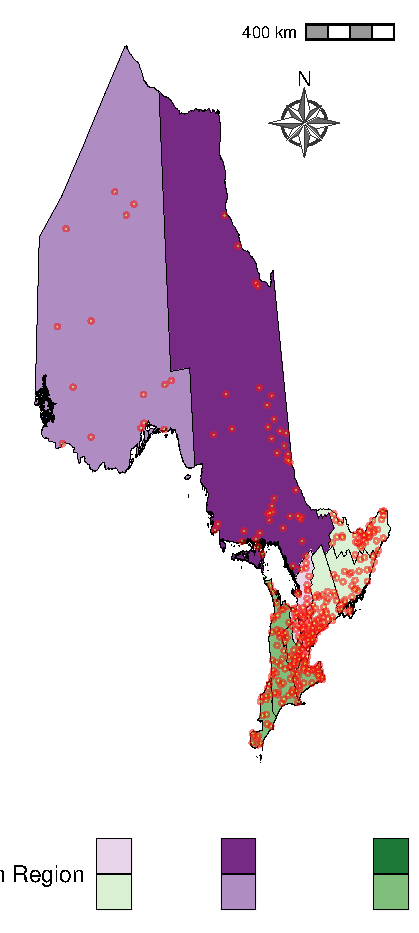
\includegraphics{../data/map_data/map.pdf}

}

\caption{\label{fig-map}Geographic representation of the data collected
by the \emph{Survey of COVID-19 related Behaviours and Attitudes},
collected by the Fields Institute in Ontario. The municipalities
(cities) from where survey participants provided answers (in the clean
dataset) appear as points. The Health six Regions are color-coded.
Internal boundaries within certain Health Regions indicate areas that
belonged to the Local Integrated Health Networks (LHINs), the geographic
areas for healthcare in Ontario before the adoption of the Health
Regions.}

\end{figure}

\hypertarget{statistical-analyses}{%
\subsection{Statistical analyses}\label{statistical-analyses}}

We used a logistic regression model to estimate the probability of
vaccination depending on the socio-economic factors described in
Table~\ref{tbl-covariates}, the Health Regions from Ontario indicated in
Section~\ref{sec-data}, and the interactions between Race and Health
Region, and Race and income, as previous studies have shown that
socio-economic factors and their interactions are significant predictors
of intent of vaccination and vaccination
status\textsuperscript{\protect\hyperlink{ref-nguyen2022}{32}--\protect\hyperlink{ref-cnat2022a}{34}}.

The model was fitted first to the clean dataset to obtain uncorrected
estimates. Additionally, because we identified differences between the
proportions of all the socio-economic factors included in the analysis
(Table~\ref{tbl-covariates}) and the Census data for Ontario, we used an
iterative proportional fitting procedure
(\emph{raking})\textsuperscript{\protect\hyperlink{ref-deming1940}{35}}
to correct the data using Census socio-economic data and Health Region
population totals, in order to obtain corrected estimates from the
model. Details regarding the correction can be found in the Appendix.
All analyses were conducted in R 4.2.2 using the packages
\texttt{survey}\textsuperscript{\protect\hyperlink{ref-lumley2011}{36}},\texttt{tidyverse}\textsuperscript{\protect\hyperlink{ref-wickham2019}{37}},
and \texttt{quarto}\textsuperscript{\protect\hyperlink{ref-quarto}{38}}.

\hypertarget{results}{%
\section{Results}\label{results}}

\hypertarget{survey-results}{%
\subsection{Survey Results}\label{survey-results}}

Table~\ref{tbl-descriptive-stats} shows the descriptive statistics from
the Fields COVID-19 survey data for vaccination status and each of the
covariates analyzed. The total number of entries analyzed was 3,551.
Overall, 26.9\% of survey respondents (958) reported not having received
the first dose of the vaccine, whereas 73.1\% (2,593) reported having
received it. Within each socio-economic factor, respondents who reported
living in a household with an income under CAD 25,000 represented 37\%
of the total number of entries, those within the CAD 25,000-59,999
income bracket represented 25\% of the total sample, and those with an
income above CAD 60,000 represented 38 \% of the sample; across all
income brackets, the percentage of individuals that reported having
received a first dose of the vaccine was consistent, above 69\%.

Within the age groups of survey respondents, the age group between 16-34
years had the highest representation in the survey responses (1,521,
42.8\% of all responses). Within this age bracket, 73\% of respondents
indicated having received the vaccine, whereas the lowest vaccination
rate was in the bracket of those 55 years of age and above, with a total
of 72\%. The Health Region with highest representation in the survey was
Toronto, accounting for 1,324 entries (37.2\%), with a vaccination rate
of 72\%. Regarding race/ethnicity, individuals that identified as
White/Caucasian represented 1313 (37\%) of all entries and had the
highest vaccination uptake with 82\% of them indicating to have received
the COVID-19 vaccine. On the other hand, the ethnic group with the
lowest number of entries in the survey was Latin American, with a total
of 180, or 5\% of all entries. Vaccination rates across all minority
groups were below the value reported by White/Caucasians, with the
lowest vaccination rate (60\%) being reported by individuals that
identified as Indigenous.

\hypertarget{tbl-descriptive-stats}{}
\begin{table}
\caption{\label{tbl-descriptive-stats}Descriptive Statistics of the Fields COVID-19 Survey (by Vaccination
Status) }\tabularnewline

\centering\begingroup\fontsize{9}{11}\selectfont

\begin{tabular}{lcc}
\toprule
\textbf{Variable} & \textbf{no}, N = 958 & \textbf{yes}, N = 2,593\\
\midrule
\textbf{Income} &  & \\
\hspace{1em}60000\_and\_above & 305 (23\%) & 1,049 (77\%)\\
\hspace{1em}25000\_59999 & 253 (28\%) & 636 (72\%)\\
\hspace{1em}under\_25000 & 400 (31\%) & 908 (69\%)\\
\textbf{Age Group} &  & \\
\hspace{1em}16\_34 & 409 (27\%) & 1,112 (73\%)\\
\hspace{1em}35\_54 & 252 (26\%) & 712 (74\%)\\
\hspace{1em}55\_and\_over & 297 (28\%) & 769 (72\%)\\
\textbf{Health Region} &  & \\
\hspace{1em}Toronto & 371 (28\%) & 953 (72\%)\\
\hspace{1em}Central & 224 (28\%) & 581 (72\%)\\
\hspace{1em}East & 135 (23\%) & 448 (77\%)\\
\hspace{1em}West & 228 (27\%) & 611 (73\%)\\
\textbf{Race} &  & \\
\hspace{1em}white\_caucasian & 233 (18\%) & 1,080 (82\%)\\
\hspace{1em}arab\_middle\_eastern & 76 (36\%) & 138 (64\%)\\
\hspace{1em}black & 114 (38\%) & 184 (62\%)\\
\hspace{1em}east\_asian\_pacific\_islander & 69 (23\%) & 234 (77\%)\\
\hspace{1em}indigenous & 76 (40\%) & 115 (60\%)\\
\hspace{1em}latin\_american & 69 (38\%) & 111 (62\%)\\
\hspace{1em}mixed & 105 (34\%) & 205 (66\%)\\
\hspace{1em}other & 128 (35\%) & 239 (65\%)\\
\hspace{1em}south\_asian & 88 (23\%) & 287 (77\%)\\
\bottomrule
\multicolumn{3}{l}{\rule{0pt}{1em}\textsuperscript{1} n (\%)}\\
\end{tabular}
\endgroup{}
\end{table}

\hypertarget{multivariate-regression}{%
\subsection{Multivariate Regression}\label{multivariate-regression}}

Table~\ref{tbl-model} shows the results of the logistic regression
models (for the uncorrected and corrected data) on vaccination status
using socio-economic factors (age group, income, race), geographical
areas (Health Regions) and the interactions between income and race and
Health Region and race. There were no statistically significant
differences in vaccination rates within the age groups from the survey,
but significant odds ratios were estimated for other covariates. Within
household income brackets, individuals with an income under CAD 25,000
or between CAD 25,000-59,999 had significantly lower odds of vaccination
than those with an income above CAD 60,000 (ORs=0.37 and 0.59,
\emph{p}=0.011 and \textless0.001, respectively). Within Race/Ethnicity,
individuals who identified as Arab/Middle Eastern, Black, or Latin
American, had significantly lower odds of vaccination than those in the
White/Caucasian group (ORs=0.31, 0.32, 0.28, and
\emph{p}=0.004,\textless0.001 and 0.004, respectively); additionally,
those individuals in the Other Race/Ethnicity group (a group that
included Southeast Asian, Filipino, West Asian, and Minorities Not
Identified Elsewhere) had even lower odds of vaccination than the other
minority groups (OR=0.22, \emph{p}\textless0.001). Regarding Health
Regions, individuals that reported living in the West Health Region
(which comprises the regions of Waterloo and Niagara, the counties of
Wellington, Essex, and Lambton, and the cities of Hamilton, Haldimand,
Brant, and Chatham-Kent) had significantly higher odds of vaccination
than those in the Health Region of Toronto (OR=1.55, \emph{p}=0.029).

Moreover, statistically-significant odd ratios were determined in the
case of the interaction of income and race; specifically, for
individuals with a household income below CAD 25,000 who identified as
Arab/Middle Eastern (OR=3.05, \emph{p}=0.013), Black (OR=3.19,
\emph{p}=0.004), Latin American (OR=2.80, \emph{p}=0.041), or that
belonged to other minority groups (OR=4.59, \emph{p}\textless0.001).
Within the CAD 25,000-59,999 income bracket, individuals who identified
as belonging to other racial minority groups had significantly higher
odds of vaccination (OR=6.93, \emph{p}\textless0.001).

For the interaction of Health Region and race, significant odds of
vaccination were identified for Black individuals in the Central Health
Region, which comprises the region of York, counties of Dufferin and
Simcoe and the district of Muskoka (OR=0.44, \emph{p}=0.046), and in
individuals that identified as part of other racial minorities or South
Asian that lived in the West Health Region (ORs=0.41, \emph{p}=0.032 and
\emph{p}=0.037, respectively).

\footnotesize
\renewcommand{\arraystretch}{0.5}

\hypertarget{tbl-model}{}
\begin{longtable}{lcccccc}
\caption{\label{tbl-model}Multiple Regression Analysis-Predictors of Vaccination Status }\tabularnewline

\toprule
\multicolumn{1}{c}{ } & \multicolumn{3}{c}{\textbf{Uncorrected}} & \multicolumn{3}{c}{\textbf{Corrected}} \\
\cmidrule(l{3pt}r{3pt}){2-4} \cmidrule(l{3pt}r{3pt}){5-7}
\textbf{Characteristic} & \textbf{OR} & \textbf{95\% CI} & \textbf{p-value} & \textbf{OR} & \textbf{95\% CI} & \textbf{p-value}\\
\midrule
\endfirsthead
\multicolumn{7}{@{}l}{\textit{(continued)}}\\
\toprule
\multicolumn{1}{c}{ } & \multicolumn{3}{c}{\textbf{Uncorrected}} & \multicolumn{3}{c}{\textbf{Corrected}} \\
\cmidrule(l{3pt}r{3pt}){2-4} \cmidrule(l{3pt}r{3pt}){5-7}
\textbf{Characteristic} & \textbf{OR} & \textbf{95\% CI} & \textbf{p-value} & \textbf{OR} & \textbf{95\% CI} & \textbf{p-value}\\
\midrule
\endhead

\endfoot
\bottomrule
\endlastfoot
\textbf{Age Group} &  &  &  &  &  & \\
\hspace{1em}16\_34 & — & — &  & — & — & \\
\hspace{1em}35\_54 & 0.93 & 0.77, 1.13 & 0.5 & 0.90 & 0.67, 1.21 & 0.5\\
\hspace{1em}55\_and\_over & 0.74 & 0.61, 0.89 & 0.002 & 0.99 & 0.74, 1.32 & >0.9\\
\textbf{Income} &  &  &  &  &  & \\
\hspace{1em}60000\_and\_above & — & — &  & — & — & \\
\hspace{1em}25000\_59999 & 0.59 & 0.41, 0.84 & 0.004 & 0.59 & 0.39, 0.89 & 0.011\\
\hspace{1em}under\_25000 & 0.41 & 0.29, 0.58 & <0.001 & 0.37 & 0.25, 0.56 & <0.001\\
\textbf{Race} &  &  &  &  &  & \\
\hspace{1em}white\_caucasian & — & — &  & — & — & \\
\hspace{1em}arab\_middle\_eastern & 0.24 & 0.12, 0.50 & <0.001 & 0.31 & 0.14, 0.69 & 0.004\\
\hspace{1em}black & 0.30 & 0.17, 0.54 & <0.001 & 0.32 & 0.17, 0.60 & <0.001\\
\hspace{1em}east\_asian\_pacific\_islander & 0.74 & 0.36, 1.52 & 0.4 & 1.15 & 0.50, 2.66 & 0.7\\
\hspace{1em}indigenous & 0.37 & 0.17, 0.81 & 0.013 & 0.44 & 0.19, 1.02 & 0.056\\
\hspace{1em}latin\_american & 0.28 & 0.13, 0.59 & <0.001 & 0.28 & 0.11, 0.67 & 0.004\\
\hspace{1em}mixed & 0.59 & 0.31, 1.12 & 0.11 & 0.64 & 0.25, 1.65 & 0.4\\
\hspace{1em}other & 0.20 & 0.11, 0.35 & <0.001 & 0.22 & 0.12, 0.41 & <0.001\\
\hspace{1em}south\_asian & 0.80 & 0.44, 1.45 & 0.5 & 0.91 & 0.49, 1.69 & 0.8\\
\textbf{Health Region} &  &  &  &  &  & \\
\hspace{1em}Toronto & — & — &  & — & — & \\
\hspace{1em}Central & 1.30 & 0.85, 2.00 & 0.2 & 1.47 & 0.92, 2.35 & 0.11\\
\hspace{1em}East & 1.54 & 1.01, 2.34 & 0.044 & 1.42 & 0.90, 2.23 & 0.13\\
\hspace{1em}West & 1.35 & 0.95, 1.94 & 0.10 & 1.55 & 1.05, 2.30 & 0.029\\
\textbf{Income * Race} &  &  &  &  &  & \\
\hspace{1em}25000\_59999 * arab\_middle\_eastern & 2.16 & 0.93, 4.99 & 0.072 & 1.79 & 0.67, 4.83 & 0.2\\
\hspace{1em}under\_25000 * arab\_middle\_eastern & 2.96 & 1.39, 6.26 & 0.005 & 3.05 & 1.26, 7.39 & 0.013\\
\hspace{1em}25000\_59999 * black & 1.19 & 0.60, 2.39 & 0.6 & 1.34 & 0.59, 3.05 & 0.5\\
\hspace{1em}under\_25000 * black & 2.88 & 1.48, 5.59 & 0.002 & 3.19 & 1.45, 6.99 & 0.004\\
\hspace{1em}25000\_59999 * east\_asian\_pacific\_islander & 0.95 & 0.44, 2.07 & >0.9 & 0.42 & 0.17, 1.05 & 0.062\\
\hspace{1em}under\_25000 * east\_asian\_pacific\_islander & 1.91 & 0.90, 4.04 & 0.090 & 1.16 & 0.47, 2.86 & 0.8\\
\hspace{1em}25000\_59999 * indigenous & 1.81 & 0.74, 4.43 & 0.2 & 1.36 & 0.48, 3.89 & 0.6\\
\hspace{1em}under\_25000 * indigenous & 1.64 & 0.73, 3.69 & 0.2 & 1.45 & 0.55, 3.80 & 0.5\\
\hspace{1em}25000\_59999 * latin\_american & 0.89 & 0.38, 2.10 & 0.8 & 1.24 & 0.45, 3.43 & 0.7\\
\hspace{1em}under\_25000 * latin\_american & 3.09 & 1.33, 7.16 & 0.009 & 2.80 & 1.04, 7.51 & 0.041\\
\hspace{1em}25000\_59999 * mixed & 0.86 & 0.39, 1.93 & 0.7 & 0.85 & 0.32, 2.26 & 0.7\\
\hspace{1em}under\_25000 * mixed & 1.26 & 0.64, 2.47 & 0.5 & 1.10 & 0.37, 3.27 & 0.9\\
\hspace{1em}25000\_59999 * other & 5.46 & 2.41, 12.3 & <0.001 & 6.93 & 2.65, 18.1 & <0.001\\
\hspace{1em}under\_25000 * other & 4.06 & 2.25, 7.31 & <0.001 & 4.59 & 2.33, 9.05 & <0.001\\
\hspace{1em}25000\_59999 * south\_asian & 1.13 & 0.54, 2.36 & 0.7 & 1.20 & 0.51, 2.85 & 0.7\\
\hspace{1em}under\_25000 * south\_asian & 1.59 & 0.83, 3.06 & 0.2 & 2.00 & 0.93, 4.30 & 0.077\\
\textbf{Race * Health Region} &  &  &  &  &  & \\
\hspace{1em}arab\_middle\_eastern * Central & 0.75 & 0.33, 1.71 & 0.5 & 0.66 & 0.26, 1.70 & 0.4\\
\hspace{1em}black * Central & 0.48 & 0.23, 1.01 & 0.055 & 0.44 & 0.19, 0.98 & 0.046\\
\hspace{1em}east\_asian\_pacific\_islander * Central & 0.84 & 0.37, 1.88 & 0.7 & 0.98 & 0.38, 2.53 & >0.9\\
\hspace{1em}indigenous * Central & 0.60 & 0.24, 1.51 & 0.3 & 0.63 & 0.22, 1.79 & 0.4\\
\hspace{1em}latin\_american * Central & 0.69 & 0.28, 1.72 & 0.4 & 0.67 & 0.23, 1.96 & 0.5\\
\hspace{1em}mixed * Central & 0.63 & 0.29, 1.35 & 0.2 & 0.73 & 0.24, 2.22 & 0.6\\
\hspace{1em}other * Central & 0.96 & 0.48, 1.92 & >0.9 & 0.80 & 0.36, 1.78 & 0.6\\
\hspace{1em}south\_asian * Central & 0.70 & 0.34, 1.45 & 0.3 & 0.54 & 0.25, 1.20 & 0.13\\
\hspace{1em}arab\_middle\_eastern * East & 0.58 & 0.20, 1.65 & 0.3 & 0.43 & 0.13, 1.45 & 0.2\\
\hspace{1em}black * East & 0.82 & 0.36, 1.86 & 0.6 & 0.83 & 0.34, 2.04 & 0.7\\
\hspace{1em}east\_asian\_pacific\_islander * East & 0.82 & 0.30, 2.24 & 0.7 & 0.86 & 0.29, 2.56 & 0.8\\
\hspace{1em}indigenous * East & 0.55 & 0.21, 1.44 & 0.2 & 0.69 & 0.23, 2.08 & 0.5\\
\hspace{1em}latin\_american * East & 0.79 & 0.28, 2.23 & 0.7 & 1.03 & 0.32, 3.34 & >0.9\\
\hspace{1em}mixed * East & 0.71 & 0.31, 1.60 & 0.4 & 0.91 & 0.28, 3.03 & 0.9\\
\hspace{1em}other * East & 0.86 & 0.37, 1.99 & 0.7 & 1.05 & 0.39, 2.83 & >0.9\\
\hspace{1em}south\_asian * East & 0.50 & 0.20, 1.24 & 0.14 & 0.52 & 0.19, 1.45 & 0.2\\
\hspace{1em}arab\_middle\_eastern * West & 1.16 & 0.48, 2.77 & 0.7 & 1.00 & 0.37, 2.73 & >0.9\\
\hspace{1em}black * West & 0.77 & 0.36, 1.65 & 0.5 & 0.76 & 0.32, 1.80 & 0.5\\
\hspace{1em}east\_asian\_pacific\_islander * West & 0.54 & 0.24, 1.20 & 0.13 & 0.52 & 0.20, 1.34 & 0.2\\
\hspace{1em}indigenous * West & 0.44 & 0.19, 1.02 & 0.056 & 0.39 & 0.14, 1.09 & 0.073\\
\hspace{1em}latin\_american * West & 0.97 & 0.39, 2.43 & >0.9 & 0.94 & 0.32, 2.72 & >0.9\\
\hspace{1em}mixed * West & 0.53 & 0.25, 1.11 & 0.092 & 0.37 & 0.12, 1.16 & 0.089\\
\hspace{1em}other * West & 0.55 & 0.27, 1.12 & 0.10 & 0.41 & 0.18, 0.93 & 0.032\\
\hspace{1em}south\_asian * West & 0.50 & 0.23, 1.07 & 0.075 & 0.41 & 0.18, 0.95 & 0.037\\*
\multicolumn{7}{l}{\rule{0pt}{1em}\textsuperscript{1} OR = Odds Ratio, CI = Confidence Interval}\\
\end{longtable}

\normalsize

\hypertarget{discussion}{%
\section{Discussion}\label{discussion}}

There existence of healthcare disparities within Ontario is a topic of
particular interest in due to the recent change in the healthcare system
of this region, which eliminated the LHIN model and adopted larger
Health Regions system in late 2019 in an attempt to address the
disparities of the former
approach\textsuperscript{\protect\hyperlink{ref-tsasis2012}{30},\protect\hyperlink{ref-dong2022}{31}}.
In this context, analyzing COVID-19 vaccination estimates within the
province is important as they can provide an initial assessment of
variations that might need to be addressed by decision-makers.

Our results indicate that across the most densely populated Health
Regions of Ontario, almost three quarters of the surveyed individuals
reported having received the first dose of the COVID-19 vaccine
(Table~\ref{tbl-descriptive-stats}). It is worth mentioning that
province-wide vaccination rates for the period of interest are somewhat
different from those of the survey, particularly in the case of those 55
years of age and older, which in the survey had a vaccination rate of
72\%, against a rate of 88.4\% reported for the closest age bracket (50
years of age and older) reported by Public Health Ontario at the start
of the period covered by the data (between September 30th, 2021 and
December 12th,
2021)\textsuperscript{\protect\hyperlink{ref-ontario-covid}{39}}. In
this regard, differences are to be expected because the survey
represents a random sample from the population, and therefore, the
sampling process is likely to cause variations between the values from
the survey and province-wide estimates.

We believe that these differences did not have a significant impact in
our analyses, because our results indicate that there were no
significant differences in vaccination odds among the age groups
considered in the survey, in agreement with the overall vaccination
rates reported for Canada, which have been relatively higher when
compared to other high income
countries\textsuperscript{\protect\hyperlink{ref-dube2022}{40}}, and
with vaccination uptake rates across different age groups presented in
other
studies\textsuperscript{\protect\hyperlink{ref-guay2022}{19},\protect\hyperlink{ref-macdonald2021}{41}}.
Moreover, vaccination rates within each age in the dataset are in good
agreement with province-wide estimates (e.g., a rate of 95\% for those
with 61 years of age, Supplementary Table A-6). Additionally, when
overall vaccination rates for the province are disaggregated, it can be
seen that regional differences were present during the period analyzed,
which can be masked by province-wide estimates. For example, the Public
Health Unit of Lambton (a region within the West Health Region) and the
Public Health Unit of Haliburton, Kawartha, and the Pine Ridge District
(an area covered by the East Health Region) reported lower vaccination
rates (78\%) for those 50 years of age and older at the beginning of the
period of interest, whereas other regions had higher vaccination
rates\textsuperscript{\protect\hyperlink{ref-ontario-covid}{39}}. To
this day, differences in vaccination rates within the province are
present, because according to Public Health Ontario, as of March of 2023
some regions have less than 75\% vaccination
rate\textsuperscript{\protect\hyperlink{ref-ontario-covid-map}{42}}.
Overall, these reasons indicate that the estimates obtained from the
data are in good agreement with the trends from the population.

We identified significant intra-provincial differences in vaccination
based on socio-economic and geographical factors. First, our results
show differences in odds of vaccination in individuals with a household
income below CAD 60,000 and in individuals belonging to visible minority
groups. Those who identified as Arab/Middle Eastern, Black, Latin
American, or that belonged to a minority group not included in the
survey (Southeast Asian, Filipino, West Asian, and minority groups not
identified elsewhere) had vaccination odds that were less than a third
of individuals that identified as White/Caucasian
(Table~\ref{tbl-model}). These results are consistent with other studies
that have shown lower vaccination rates in individuals that identify as
part of a racial minority, or that have a low household
income\textsuperscript{\protect\hyperlink{ref-guay2022}{19}--\protect\hyperlink{ref-hussain2022}{21},\protect\hyperlink{ref-carter2022}{43}}.

In this study, we also decided to explore the interactions between
income and race and race and Health Region, as it is known that many
individuals within racial minority groups perform tend to occupy certain
types of occupations that fall within income brackets that have been
shown to be associated with differences in vaccination uptake. In other
words, we decided to explore if there were differences in vaccination
within racial groups in certain income brackets and in certain the
Health Regions. In this regard, it is interesting to note that although
overall self-reported vaccination rates were found to be statistically
significantly lower in various racial minority groups when compared to
White/Caucasian individuals (Table~\ref{tbl-model}), the change in odds
of vaccination within certain racial groups and income strata was
actually positive, in contrast to the White/Caucasian group, for which
vaccination odds decreased in lower income brackets (when compared to
the CAD 60,000 and over bracket, Supplementary Figure A-3). More
specifically, the change in odds of vaccination increased in individuals
who identified as Arab/Middle Eastern, Black, Latin American, or
belonging to other minority groups with a household income below CAD
25,000, which was also true for individuals in other racial minority
groups with an income between CAD 25,000-59,999 (Table~\ref{tbl-model},
Supplementary Figure A-3).

This result is likely due to the fact that individuals that belong
racial minority groups tend to perform occupations that have been deemed
as ``essential'' in the context of the
pandemic\textsuperscript{\protect\hyperlink{ref-hawkins2020}{44},\protect\hyperlink{ref-ct2021}{45}},
which include occupations such as grocery store workers, gas station
workers, warehouse and distribution workers, and manufacturing workers,
all being occupations for which an income within the significant
brackets is to be expected. In the case of Ontario, essential workers
had priority for COVID-19
vaccination\textsuperscript{\protect\hyperlink{ref-mishra2021}{46}},
which would explain the higher odds of vaccination for these individuals
in certain income brackets, in contrast to the lower odds of vaccination
for the same type of individuals with higher household income. In other
words, it is possible that the type of occupation played an important
role in increasing the odds of vaccination in these racial minority
groups.

Additionally, significant higher vaccination odds were identified in the
West Health Region when compared to the Health Region of Toronto
(Table~\ref{tbl-model}). The West Health Region comprises the regions of
Waterloo and Niagara, the counties of Wellington, Essex and Lambton, and
the cities of Hamilton, Haldimand, Brant, and Chatham-Kent. In this
case, a possible rationale for the results is the fact that in the
survey, about 47\% of the entries for this Health Region corresponded to
White/Caucasian individuals, who reported an overall 83\% vaccination
rate (Supplementary Table A-7). However, the interaction effect of
Health Region and race was also significant in the case of individuals
identifying as South Asian or other minorities not included in the
survey Table~\ref{tbl-model}. In this case, the results of the
interaction term in the model indicate that the odds of vaccination for
those within the South Asian and Other minority groups in the West
Region decreased when compared to the other Health Regions
(Supplementary Figure A-4).

According to Ontario Health, 13.2\% of the population in the West Health
Region identifies as a visible minority, whereas 2.5\% identifies as
Indigenous\textsuperscript{\protect\hyperlink{ref-ontariohealth}{47}}.
In the case of this analysis, the estimated lower odds are likely to be
explained from a socio-economic perspective. In fact, 50\% of the
answers from this region in the survey came from the former LHINs of
Hamilton Niagara Haldimand Brant, and Erie St.~Clair, both which are
among the regions of Ontario with the highest proportion of their
population (more than 20\%) in the lowest income
quintile\textsuperscript{\protect\hyperlink{ref-buajitti2018}{48}}
(Supplementary Table A-8). Therefore, this result partly reinforces the
well-known existing association between low vaccination rates and
income, but it additionally indicates that there were intra-regional
differences in vaccination. Interestingly, a disproportionate number of
COVID-19 cases and low vaccination rate (under 50\%) have been
previously reported in the South Asian community of
Ontario\textsuperscript{\protect\hyperlink{ref-anand2022}{49}}; in this
regard, our result provides additional context by showing that within
the South Asian community, there were differences in vaccination uptake
across Ontario. Moreover, because significant lower odds of vaccination
were also identified other minority groups, this provides a rationale
for future studies that explore how vaccination uptake varies across
different minority groups within Ontario and other Canadian provinces.

There are some limitations to the present study. First, the data
collection design, which allowed respondents to withdraw from the survey
at any point, resulted in a high number of unique entries in the survey
with multiple missing answers. Because we focused on entries that had
complete observations in the covariates of interest for our analysis, it
is possible that some information was not considered by excluding
observations that had information in other variables (such as work from
home, or number of persons in the household). However, we attempted to
minimize this possibility by correcting the dataset using information
from the Census. More granular corrections, which for example could be
based on demographic information by municipality, could be used in the
future to obtain a more accurate approximation to the population totals
of the province. Moreover, our analysis did not consider the North West
and North East Health Regions, due to the low number of entries from
these areas in the survey (Figure~\ref{fig-map}). Although low
representation from these areas is based on the fact that these regions
only account for 5\% of the total population of Ontario, these regions
are the home to more than 100,000 individuals that identify as
Indigenous\textsuperscript{\protect\hyperlink{ref-ontariohealth}{47}}, a
minority group that has historically suffered from reduced access to
health care and
discrimination\textsuperscript{\protect\hyperlink{ref-mosby2021}{17}}.
Therefore, there is a need for additional studies that focus on these
low-populated Health Regions in Ontario where disparities in vaccination
might be significant and understudied.

The results in this study are based on self-reported data, where there
is a risk that biased values are reported. Despite this, because in the
context of COVID-19 it has been shown that good agreement exists between
self-reported and documented vaccination
status\textsuperscript{\protect\hyperlink{ref-stephenson2022}{50}}, and
therefore, the effect of self-reported bias is likely to not be
significant in our analyses. Finally, it is likely that there have been
differences in vaccination across the province as more doses of the
vaccine were administered and as successive variants emerged. Because
this study focused only on vaccination status regarding the first dose
of the vaccine within a relatively short time window, it can only
provide a snapshot of the societal dynamics behind the pandemic.
Nonetheless, the results presented here can serve as a starting point to
motivate the collection of robust longitudinal data that can be used to
quantify geographical and temporal differences within vulnerable
segments of the population, and that can be used to inform the
development of adequate public health policies within the province of
Ontario or across other provinces that aim to minimize disparities in
health access.

\hypertarget{conclusion}{%
\section{Conclusion}\label{conclusion}}

This study explored differences in COVID-19 vaccination across the
province of Ontario between late 2021 and early 2022 by taking into
consideration socio-economic factors, such as income and race, their
interactions, and the Health Regions within the province. Our results
show that, during the period analyzed, significant differences in
vaccination existed across different visible minority groups, income
brackets, and Health Regions, showing intra-provincial disparities in
vaccine uptake. As the COVID-19 continues around the world, it important
that future public policies take into consideration how to adequately
reach individuals within minority groups that live across geographical
areas where less probabilities of being vaccinated are likely. At the
moment, this is an ongoing issue that needs to be addressed to ensure a
more homogeneous outcome from the pandemic.

\hypertarget{references}{%
\section{References}\label{references}}

\hypertarget{refs}{}
\begin{CSLReferences}{0}{0}
\leavevmode\vadjust pre{\hypertarget{ref-davis2022}{}}%
\CSLLeftMargin{1. }%
\CSLRightInline{Davis CJ, Golding M, McKay R. Efficacy information
influences intention to take COVID-19 vaccine. \emph{British Journal of
Health Psychology}. 2022;27(2):300-319.
doi:\url{https://doi.org/10.1111/bjhp.12546}}

\leavevmode\vadjust pre{\hypertarget{ref-bogoch2022}{}}%
\CSLLeftMargin{2. }%
\CSLRightInline{Bogoch II, Halani S. {COVID}-19 vaccines: A geographic,
social and policy view of vaccination efforts in ontario, canada.
\emph{Cambridge Journal of Regions, Economy and Society}. Published
online November 2022.
doi:\href{https://doi.org/10.1093/cjres/rsac043}{10.1093/cjres/rsac043}}

\leavevmode\vadjust pre{\hypertarget{ref-tanne2020}{}}%
\CSLLeftMargin{3. }%
\CSLRightInline{Tanne JH. Covid-19: {FDA} panel votes to authorise
pfizer {BioNTech} vaccine. \emph{{BMJ}}. Published online December
2020:m4799.
doi:\href{https://doi.org/10.1136/bmj.m4799}{10.1136/bmj.m4799}}

\leavevmode\vadjust pre{\hypertarget{ref-thelancet2021}{}}%
\CSLLeftMargin{4. }%
\CSLRightInline{Microbe TL. {COVID}-19 vaccines: The pandemic will not
end overnight. \emph{The Lancet Microbe}. 2021;2(1):e1.
doi:\href{https://doi.org/10.1016/s2666-5247(20)30226-3}{10.1016/s2666-5247(20)30226-3}}

\leavevmode\vadjust pre{\hypertarget{ref-watson2022}{}}%
\CSLLeftMargin{5. }%
\CSLRightInline{Watson OJ, Barnsley G, Toor J, Hogan AB, Winskill P,
Ghani AC. Global impact of the first year of {COVID}-19 vaccination: A
mathematical modelling study. \emph{The Lancet Infectious Diseases}.
2022;22(9):1293-1302.
doi:\href{https://doi.org/10.1016/s1473-3099(22)00320-6}{10.1016/s1473-3099(22)00320-6}}

\leavevmode\vadjust pre{\hypertarget{ref-kayser2021}{}}%
\CSLLeftMargin{6. }%
\CSLRightInline{Kayser V, Ramzan I. Vaccines and vaccination: History
and emerging issues. \emph{Human Vaccines {\&}amp\(\mathsemicolon\)
Immunotherapeutics}. 2021;17(12):5255-5268.
doi:\href{https://doi.org/10.1080/21645515.2021.1977057}{10.1080/21645515.2021.1977057}}

\leavevmode\vadjust pre{\hypertarget{ref-li2021}{}}%
\CSLLeftMargin{7. }%
\CSLRightInline{Li Q, Wang J, Tang Y, Lu H. Next-generation COVID-19
vaccines: Opportunities for vaccine development and challenges in
tackling COVID-19. \emph{Drug Discoveries \& Therapeutics}.
2021;15(3):118-123.
doi:\href{https://doi.org/10.5582/ddt.2021.0105}{10.5582/ddt.2021.0105}}

\leavevmode\vadjust pre{\hypertarget{ref-gerretsen2021}{}}%
\CSLLeftMargin{8. }%
\CSLRightInline{Gerretsen P, Kim J, Caravaggio F, et al. Individual
determinants of {COVID}-19 vaccine hesitancy. Inbaraj LR, ed.
\emph{{PLOS} {ONE}}. 2021;16(11):e0258462.
doi:\href{https://doi.org/10.1371/journal.pone.0258462}{10.1371/journal.pone.0258462}}

\leavevmode\vadjust pre{\hypertarget{ref-tamey2022}{}}%
\CSLLeftMargin{9. }%
\CSLRightInline{Yamey G, Garcia P, Hassan F, et al. It is not too late
to achieve global covid-19 vaccine equity. \emph{{BMJ}}. Published
online March 2022:e070650.
doi:\href{https://doi.org/10.1136/bmj-2022-070650}{10.1136/bmj-2022-070650}}

\leavevmode\vadjust pre{\hypertarget{ref-nafilyan2021}{}}%
\CSLLeftMargin{10. }%
\CSLRightInline{Nafilyan V, Dolby T, Razieh C, et al. Sociodemographic
inequality in {COVID}-19 vaccination coverage among elderly adults in
england: A national linked data study. \emph{{BMJ} Open}.
2021;11(7):e053402.
doi:\href{https://doi.org/10.1136/bmjopen-2021-053402}{10.1136/bmjopen-2021-053402}}

\leavevmode\vadjust pre{\hypertarget{ref-malik2020}{}}%
\CSLLeftMargin{11. }%
\CSLRightInline{Malik AA, McFadden SM, Elharake J, Omer SB. Determinants
of {COVID}-19 vaccine acceptance in the {US}.
\emph{{EClinicalMedicine}}. 2020;26:100495.
doi:\href{https://doi.org/10.1016/j.eclinm.2020.100495}{10.1016/j.eclinm.2020.100495}}

\leavevmode\vadjust pre{\hypertarget{ref-willis2021}{}}%
\CSLLeftMargin{12. }%
\CSLRightInline{Willis DE, Andersen JA, Bryant-Moore K, et al.
{COVID}-19 vaccine hesitancy: Race/ethnicity, trust, and fear.
\emph{Clinical and Translational Science}. 2021;14(6):2200-2207.
doi:\href{https://doi.org/10.1111/cts.13077}{10.1111/cts.13077}}

\leavevmode\vadjust pre{\hypertarget{ref-skirrow2022}{}}%
\CSLLeftMargin{13. }%
\CSLRightInline{Skirrow H, Barnett S, Bell S, et al. Women's views on
accepting {COVID}-19 vaccination during and after pregnancy, and for
their babies: A multi-methods study in the {UK}. \emph{{BMC} Pregnancy
and Childbirth}. 2022;22(1).
doi:\href{https://doi.org/10.1186/s12884-021-04321-3}{10.1186/s12884-021-04321-3}}

\leavevmode\vadjust pre{\hypertarget{ref-stoler2021}{}}%
\CSLLeftMargin{14. }%
\CSLRightInline{Stoler J, Enders AM, Klofstad CA, Uscinski JE. The
limits of medical trust in mitigating {COVID}-19 vaccine hesitancy among
black americans. \emph{Journal of General Internal Medicine}.
2021;36(11):3629-3631.
doi:\href{https://doi.org/10.1007/s11606-021-06743-3}{10.1007/s11606-021-06743-3}}

\leavevmode\vadjust pre{\hypertarget{ref-khubchandani2021}{}}%
\CSLLeftMargin{15. }%
\CSLRightInline{Khubchandani J, Sharma S, Price JH, Wiblishauser MJ,
Sharma M, Webb FJ. {COVID}-19 vaccination hesitancy in the united
states: A rapid national assessment. \emph{Journal of Community Health}.
2021;46(2):270-277.
doi:\href{https://doi.org/10.1007/s10900-020-00958-x}{10.1007/s10900-020-00958-x}}

\leavevmode\vadjust pre{\hypertarget{ref-bogart2021}{}}%
\CSLLeftMargin{16. }%
\CSLRightInline{Bogart LM, Ojikutu BO, Tyagi K, et al. {COVID}-19
related medical mistrust, health impacts, and potential vaccine
hesitancy among black americans living with {HIV}. \emph{{JAIDS} Journal
of Acquired Immune Deficiency Syndromes}. 2021;86(2):200-207.
doi:\href{https://doi.org/10.1097/qai.0000000000002570}{10.1097/qai.0000000000002570}}

\leavevmode\vadjust pre{\hypertarget{ref-mosby2021}{}}%
\CSLLeftMargin{17. }%
\CSLRightInline{Mosby I, Swidrovich J. Medical experimentation and the
roots of {COVID}-19 vaccine hesitancy among indigenous peoples in
canada. \emph{Canadian Medical Association Journal}.
2021;193(11):E381-E383.
doi:\href{https://doi.org/10.1503/cmaj.210112}{10.1503/cmaj.210112}}

\leavevmode\vadjust pre{\hypertarget{ref-freeman2020}{}}%
\CSLLeftMargin{18. }%
\CSLRightInline{Freeman D, Loe BS, Chadwick A, et al. {COVID}-19 vaccine
hesitancy in the {UK}: The oxford coronavirus explanations, attitudes,
and narratives survey (oceans) {II}. \emph{Psychological Medicine}.
2020;52(14):3127-3141.
doi:\href{https://doi.org/10.1017/s0033291720005188}{10.1017/s0033291720005188}}

\leavevmode\vadjust pre{\hypertarget{ref-guay2022}{}}%
\CSLLeftMargin{19. }%
\CSLRightInline{Guay M, Maquiling A, Chen R, et al. Measuring
inequalities in {COVID}-19 vaccination uptake and intent: Results from
the canadian community health survey 2021. \emph{{BMC} Public Health}.
2022;22(1).
doi:\href{https://doi.org/10.1186/s12889-022-14090-z}{10.1186/s12889-022-14090-z}}

\leavevmode\vadjust pre{\hypertarget{ref-muhajarine2021}{}}%
\CSLLeftMargin{20. }%
\CSLRightInline{Muhajarine N, Adeyinka DA, McCutcheon J, Green KL,
Fahlman M, Kallio N. {COVID}-19 vaccine hesitancy and refusal and
associated factors in an adult population in saskatchewan, canada:
Evidence from predictive modelling. Gesser-Edelsburg A, ed. \emph{{PLOS}
{ONE}}. 2021;16(11):e0259513.
doi:\href{https://doi.org/10.1371/journal.pone.0259513}{10.1371/journal.pone.0259513}}

\leavevmode\vadjust pre{\hypertarget{ref-hussain2022}{}}%
\CSLLeftMargin{21. }%
\CSLRightInline{Hussain B, Latif A, Timmons S, Nkhoma K, Nellums LB.
Overcoming {COVID}-19 vaccine hesitancy among ethnic minorities: A
systematic review of {UK} studies. \emph{Vaccine}.
2022;40(25):3413-3432.
doi:\href{https://doi.org/10.1016/j.vaccine.2022.04.030}{10.1016/j.vaccine.2022.04.030}}

\leavevmode\vadjust pre{\hypertarget{ref-nguyen2021}{}}%
\CSLLeftMargin{22. }%
\CSLRightInline{Nguyen KH, Nguyen K, Corlin L, Allen JD, Chung M.
Changes in {COVID}-19 vaccination receipt and intention to vaccinate by
socioeconomic characteristics and geographic area, united states,
january 6 {\textendash} march 29, 2021. \emph{Annals of Medicine}.
2021;53(1):1419-1428.
doi:\href{https://doi.org/10.1080/07853890.2021.1957998}{10.1080/07853890.2021.1957998}}

\leavevmode\vadjust pre{\hypertarget{ref-mollalo2021}{}}%
\CSLLeftMargin{23. }%
\CSLRightInline{Mollalo A, Tatar M. Spatial modeling of {COVID}-19
vaccine hesitancy in the united states. \emph{International Journal of
Environmental Research and Public Health}. 2021;18(18):9488.
doi:\href{https://doi.org/10.3390/ijerph18189488}{10.3390/ijerph18189488}}

\leavevmode\vadjust pre{\hypertarget{ref-yang2022}{}}%
\CSLLeftMargin{24. }%
\CSLRightInline{Yang TC, Matthews SA, Sun F. Multiscale dimensions of
spatial process: {COVID}-19 fully vaccinated rates in u.s. counties.
\emph{American Journal of Preventive Medicine}. 2022;63(6):954-961.
doi:\href{https://doi.org/10.1016/j.amepre.2022.06.006}{10.1016/j.amepre.2022.06.006}}

\leavevmode\vadjust pre{\hypertarget{ref-tiu2022}{}}%
\CSLLeftMargin{25. }%
\CSLRightInline{Tiu A, Susswein Z, Merritt A, Bansal S. Characterizing
the spatiotemporal heterogeneity of the {COVID}-19 vaccination
landscape. \emph{American Journal of Epidemiology}.
2022;191(10):1792-1802.
doi:\href{https://doi.org/10.1093/aje/kwac080}{10.1093/aje/kwac080}}

\leavevmode\vadjust pre{\hypertarget{ref-bhuiyan2022}{}}%
\CSLLeftMargin{26. }%
\CSLRightInline{Bhuiyan MAN, Davis TC, Arnold CL, et al. Using the
social vulnerability index to assess {COVID}-19 vaccine uptake in
louisiana. \emph{{GeoJournal}}. Published online December 2022.
doi:\href{https://doi.org/10.1007/s10708-022-10802-5}{10.1007/s10708-022-10802-5}}

\leavevmode\vadjust pre{\hypertarget{ref-wood2022}{}}%
\CSLLeftMargin{27. }%
\CSLRightInline{Wood AJ, MacKintosh AM, Stead M, Kao RR. Predicting
future spatial patterns in {COVID}-19 booster vaccine uptake. Published
online September 2022.
doi:\href{https://doi.org/10.1101/2022.08.30.22279415}{10.1101/2022.08.30.22279415}}

\leavevmode\vadjust pre{\hypertarget{ref-choi2021}{}}%
\CSLLeftMargin{28. }%
\CSLRightInline{Choi KH, Denice PA, Ramaj S. Vaccine and {COVID}-19
trajectories. \emph{Socius: Sociological Research for a Dynamic World}.
2021;7:237802312110529.
doi:\href{https://doi.org/10.1177/23780231211052946}{10.1177/23780231211052946}}

\leavevmode\vadjust pre{\hypertarget{ref-mckinnon2021}{}}%
\CSLLeftMargin{29. }%
\CSLRightInline{McKinnon B, Quach C, Dubé Ève, Nguyen CT, Zinszer K.
Social inequalities in {COVID}-19 vaccine acceptance and uptake for
children and adolescents in montreal, canada. \emph{Vaccine}.
2021;39(49):7140-7145.
doi:\href{https://doi.org/10.1016/j.vaccine.2021.10.077}{10.1016/j.vaccine.2021.10.077}}

\leavevmode\vadjust pre{\hypertarget{ref-tsasis2012}{}}%
\CSLLeftMargin{30. }%
\CSLRightInline{Tsasis P, Evans JM, Owen S. Reframing the challenges to
integrated care: A complex-adaptive systems perspective.
\emph{International Journal of Integrated Care}. 2012;12(5).
doi:\href{https://doi.org/10.5334/ijic.843}{10.5334/ijic.843}}

\leavevmode\vadjust pre{\hypertarget{ref-dong2022}{}}%
\CSLLeftMargin{31. }%
\CSLRightInline{Dong L, Sahu R, Black R. Governance in the
transformational journey toward integrated healthcare: The case of
ontario. \emph{Journal of Information Technology Teaching Cases}.
Published online December 2022:204388692211473.
doi:\href{https://doi.org/10.1177/20438869221147313}{10.1177/20438869221147313}}

\leavevmode\vadjust pre{\hypertarget{ref-nguyen2022}{}}%
\CSLLeftMargin{32. }%
\CSLRightInline{Nguyen KH, Anneser E, Toppo A, Allen JD, Parott JS,
Corlin L. Disparities in national and state estimates of {COVID}-19
vaccination receipt and intent to vaccinate by race/ethnicity, income,
and age group among adults~\(\geq\)~18~years, united states.
\emph{Vaccine}. 2022;40(1):107-113.
doi:\href{https://doi.org/10.1016/j.vaccine.2021.11.040}{10.1016/j.vaccine.2021.11.040}}

\leavevmode\vadjust pre{\hypertarget{ref-shih2021}{}}%
\CSLLeftMargin{33. }%
\CSLRightInline{Shih SF, Wagner AL, Masters NB, Prosser LA, Lu Y,
Zikmund-Fisher BJ. Vaccine hesitancy and rejection of a vaccine for the
novel coronavirus in the united states. \emph{Frontiers in Immunology}.
2021;12.
doi:\href{https://doi.org/10.3389/fimmu.2021.558270}{10.3389/fimmu.2021.558270}}

\leavevmode\vadjust pre{\hypertarget{ref-cnat2022a}{}}%
\CSLLeftMargin{34. }%
\CSLRightInline{Cénat JM, Noorishad PG, Farahi SMMM, et al. Prevalence
and factors related to {COVID}-19 vaccine hesitancy and unwillingness in
canada: A systematic review and meta-analysis. \emph{Journal of Medical
Virology}. 2022;95(1).
doi:\href{https://doi.org/10.1002/jmv.28156}{10.1002/jmv.28156}}

\leavevmode\vadjust pre{\hypertarget{ref-deming1940}{}}%
\CSLLeftMargin{35. }%
\CSLRightInline{Deming WE, Stephan FF. On a least squares adjustment of
a sampled frequency table when the expected marginal totals are known.
\emph{The Annals of Mathematical Statistics}. 1940;11(4):427-444.
doi:\href{https://doi.org/10.1214/aoms/1177731829}{10.1214/aoms/1177731829}}

\leavevmode\vadjust pre{\hypertarget{ref-lumley2011}{}}%
\CSLLeftMargin{36. }%
\CSLRightInline{Lumley T. \emph{Complex Surveys}. John Wiley \& Sons;
2011.}

\leavevmode\vadjust pre{\hypertarget{ref-wickham2019}{}}%
\CSLLeftMargin{37. }%
\CSLRightInline{Wickham H, Averick M, Bryan J, et al. Welcome to the
{tidyverse}. \emph{Journal of Open Source Software}. 2019;4(43):1686.
doi:\href{https://doi.org/10.21105/joss.01686}{10.21105/joss.01686}}

\leavevmode\vadjust pre{\hypertarget{ref-quarto}{}}%
\CSLLeftMargin{38. }%
\CSLRightInline{Allaire J. \emph{Quarto: R Interface to 'Quarto'
Markdown Publishing System}.; 2022.
\url{https://CRAN.R-project.org/package=quarto}}

\leavevmode\vadjust pre{\hypertarget{ref-ontario-covid}{}}%
\CSLLeftMargin{39. }%
\CSLRightInline{{Ontario COVID-19 Data Tool}. Accessed February 27,
2023.
\url{https://www.publichealthontario.ca/en/data-and-analysis/infectious-disease/covid-19-data-surveillance/covid-19-data-tool?tab=vaccine}}

\leavevmode\vadjust pre{\hypertarget{ref-dube2022}{}}%
\CSLLeftMargin{40. }%
\CSLRightInline{Dubé E, Gagnon D, MacDonald N. Between persuasion and
compulsion: The case of {COVID}-19 vaccination in canada.
\emph{Vaccine}. 2022;40(29):3923-3926.
doi:\href{https://doi.org/10.1016/j.vaccine.2022.05.053}{10.1016/j.vaccine.2022.05.053}}

\leavevmode\vadjust pre{\hypertarget{ref-macdonald2021}{}}%
\CSLLeftMargin{41. }%
\CSLRightInline{MacDonald NE, Comeau J, Dubé Ève, et al. Royal society
of canada {COVID}-19 report: Enhancing {COVID}-19 vaccine acceptance in
canada. Blais JM, ed. \emph{{FACETS}}. 2021;6:1184-1246.
doi:\href{https://doi.org/10.1139/facets-2021-0037}{10.1139/facets-2021-0037}}

\leavevmode\vadjust pre{\hypertarget{ref-ontario-covid-map}{}}%
\CSLLeftMargin{42. }%
\CSLRightInline{{Ontario COVID-19 Data Tool}. Accessed March 24, 2023.
\url{https://www.publichealthontario.ca/en/data-and-analysis/infectious-disease/covid-19-data-surveillance/covid-19-data-tool?tab=maps}}

\leavevmode\vadjust pre{\hypertarget{ref-carter2022}{}}%
\CSLLeftMargin{43. }%
\CSLRightInline{Carter MA, Biro S, Maier A, Shingler C, Guan TH.
{COVID}-19 vaccine uptake in southeastern ontario, canada: Monitoring
and addressing health inequities. \emph{Journal of Public Health
Management and Practice}. 2022;28(6):615-623.
doi:\href{https://doi.org/10.1097/phh.0000000000001565}{10.1097/phh.0000000000001565}}

\leavevmode\vadjust pre{\hypertarget{ref-hawkins2020}{}}%
\CSLLeftMargin{44. }%
\CSLRightInline{Hawkins D. Differential occupational risk for {COVID}-19
and other infection exposure according to race and ethnicity.
\emph{American Journal of Industrial Medicine}. 2020;63(9):817-820.
doi:\href{https://doi.org/10.1002/ajim.23145}{10.1002/ajim.23145}}

\leavevmode\vadjust pre{\hypertarget{ref-ct2021}{}}%
\CSLLeftMargin{45. }%
\CSLRightInline{Côté D, Durant S, MacEachen E, et al. A rapid scoping
review of {COVID}-19 and vulnerable workers: Intersecting occupational
and public health issues. \emph{American Journal of Industrial
Medicine}. 2021;64(7):551-566.
doi:\href{https://doi.org/10.1002/ajim.23256}{10.1002/ajim.23256}}

\leavevmode\vadjust pre{\hypertarget{ref-mishra2021}{}}%
\CSLLeftMargin{46. }%
\CSLRightInline{Mishra S, Stall NM, Ma H, et al. \emph{A Vaccination
Strategy for Ontario {COVID}-19 Hotspots and Essential Workers}. Ontario
{COVID}-19 Science Advisory Table; 2021.
doi:\href{https://doi.org/10.47326/ocsat.2021.02.26.1.0}{10.47326/ocsat.2021.02.26.1.0}}

\leavevmode\vadjust pre{\hypertarget{ref-ontariohealth}{}}%
\CSLLeftMargin{47. }%
\CSLRightInline{\emph{{A}nnual {B}usiness {P}lan 2022/23}. Ontario
Health;
\url{https://www.ontariohealth.ca/sites/ontariohealth/files/2022-05/OHBusinessPlan22_23.pdf};
2022.}

\leavevmode\vadjust pre{\hypertarget{ref-buajitti2018}{}}%
\CSLLeftMargin{48. }%
\CSLRightInline{Buajitti E, Watson T, Kornas K, Bornbaum C, Henry D,
Rosella LC. Ontario atlas of adult mortality, 1992-2015: Trends in
{L}ocal {H}ealth {I}ntegration {N}etworks. Published online 2018.
\url{https://tspace.library.utoronto.ca/handle/1807/82836}}

\leavevmode\vadjust pre{\hypertarget{ref-anand2022}{}}%
\CSLLeftMargin{49. }%
\CSLRightInline{Anand SS, Arnold C, Bangdiwala SI, et al. Seropositivity
and risk factors for {SARS}-{CoV}-2 infection in a south asian community
in ontario: A cross-sectional analysis of a prospective cohort study.
\emph{{CMAJ} Open}. 2022;10(3):E599-E609.
doi:\href{https://doi.org/10.9778/cmajo.20220031}{10.9778/cmajo.20220031}}

\leavevmode\vadjust pre{\hypertarget{ref-stephenson2022}{}}%
\CSLLeftMargin{50. }%
\CSLRightInline{Stephenson M, Olson SM, Self WH, et al. Ascertainment of
vaccination status by self-report versus source documentation: Impact on
measuring {COVID}-19 vaccine effectiveness. \emph{Influenza and Other
Respiratory Viruses}. 2022;16(6):1101-1111.
doi:\href{https://doi.org/10.1111/irv.13023}{10.1111/irv.13023}}

\end{CSLReferences}



\end{document}
